% =====================================================================
%  QAI-SAGIN @ AICON 2026 — full paper (12-16 trang), Springer LNICST
%
%  ⛔ BA DIEU KIEN tu claim-structure.md, bo mot cai la hong:
%   DK1  KHONG nhac lai tuyen bo ly thuyet "QI la EDA" cua qi-insight (da bi Platel 2009 chiem)
%   DK2  KHONG them ham chuan tong hop nao (Rastrigin...). Chi bai toan NTN that.
%   DK3  PHAI trich kho da phat hanh cua nhom, nhung o NGOI THU BA vi review la DOUBLE-BLIND
%
%  ⚠ KHONG GO SO. Moi con so den tu figures/out/numbers.tex, sinh tu results/*.json.
%  Chay: python3 code/a2_underpowered.py && python3 figures/make_figures.py
% =====================================================================
\documentclass[runningheads]{llncs}

\usepackage[T1]{fontenc}
\usepackage[utf8]{inputenc}
\usepackage{graphicx}
\usepackage{booktabs}
\usepackage{amsmath,amssymb}
\usepackage{siunitx}
\usepackage{xcolor}
\usepackage[hidelinks]{hyperref}

\newcommand{\numBudget}{20.000}
\newcommand{\numCells}{48}
\newcommand{\numCellsMulti}{24}
\newcommand{\numInst}{3}
\newcommand{\numMinSpread}{1}
\newcommand{\numMultiEffectRatio}{0.70}
\newcommand{\numMultiLoss}{64}
\newcommand{\numMultiLossPct}{98}
\newcommand{\numMultiTie}{1}
\newcommand{\numMultiTiePct}{2}
\newcommand{\numMultiUnits}{65}
\newcommand{\numMultiWin}{0}
\newcommand{\numQpsoWinTotal}{0}
\newcommand{\numRestartBest}{144}
\newcommand{\numSeeds}{30}
\newcommand{\numSpikeG}{0,30}
\newcommand{\numSpikeInst}{3}
\newcommand{\numSpikeK}{8}
\newcommand{\numSpikeKappa}{0,05}
\newcommand{\numSpikeMulti}{0}
\newcommand{\numStarts}{30}
\newcommand{\numUniEffectRatio}{0.27}
\newcommand{\numUniLoss}{15}
\newcommand{\numUniLossPct}{19}
\newcommand{\numUniTie}{64}
\newcommand{\numUniTiePct}{81}
\newcommand{\numUniUnits}{79}
\newcommand{\numUniWin}{0}
\newcommand{\numUnits}{144}


\begin{document}

\title{Where You Screen Decides What You Conclude:\\
Instance Space Analysis for Quantum-Inspired\\ Resource Allocation in Non-Terrestrial Networks}

% ⚠ DOUBLE-BLIND: khong ten tac gia, khong don vi, khong URL kho cua nhom.
\author{Anonymous Submission}
\institute{Paper ID (to be assigned)}

\maketitle

\begin{abstract}
Quantum-inspired (QI) metaheuristics are widely proposed for resource allocation in
space-air-ground integrated networks, and the evidence offered for them is usually a comparison
on a handful of problem configurations, against a small set of population-based baselines, over
few repetitions. We ask what changes when three evaluation conventions that are already standard
in neighbouring communities are applied together to one concrete non-terrestrial problem: mapping
the instance space rather than sampling one point in it, giving every method the same
function-evaluation budget with restarts permitted, and reporting a method effect against the
spread the random seed alone produces. On a multi-beam power allocation problem we map
\numCells{} configurations with \numInst{} instances each and compare four optimisers over
\numSeeds{} seeds at a matched budget of \numBudget{} evaluations, for \numUnits{} units in
total. Four results follow. First, \numCellsMulti{} of \numCells{} configurations are multimodal,
and multimodality is driven almost entirely by amplifier distortion rather than by interference
or beam count, rising from \numKnobKappaLo\% to \numKnobKappaHi\% of units across that one knob.
Second, across all four optimisers restart local search is best or tied in \numRestartBest{} of
\numUnits{} units, ahead of the QI method (\numBestQpso{}), CMA-ES (\numBestCmaes{}) and
differential evolution (\numBestDe{}); and against the usual argument for population-based
search, the QI method ties restart local search on \numUniTiePct\% of unimodal units while
losing on \numMultiLossPct\% of multimodal ones. Third, every effect we measure is smaller than the seed-induced spread while its direction
never once reverses across \numUnits{} units. Fourth, reconstructing \numStudies{} studies at the
size typically reported, we find the headline is decided by two choices of the experimenter
rather than by the problem: against differential evolution \numSmallDeAhead\% of such studies
report the QI method ahead, against restart local search \numSmallRestartBehind\% report it
behind, and among studies that happen to screen only unimodal configurations \numAllUniTie\%
report no difference at all. We release the map and the harness.
\keywords{Quantum-inspired optimisation \and Non-terrestrial networks \and Instance space
analysis \and Benchmarking \and Reproducibility \and Resource allocation.}
\end{abstract}

% =====================================================================
\section{Introduction}

Space-air-ground integrated networks (SAGINs) combine low Earth orbit constellations,
high-altitude platforms, unmanned aerial vehicles and terrestrial cells into one programmable
fabric, and non-terrestrial networks (NTN) are now a first-class component of the 3GPP releases.
The control problems these systems pose share a shape: beam steering, handover, slice placement,
trajectory planning and spectrum assignment all produce decision spaces that grow rapidly with
the number of nodes, and all must be solved under severe energy and latency budgets. That shape
is an invitation to metaheuristics, and quantum-inspired (QI) methods are among the families most
frequently proposed for it, on the argument that they bring a complementary search behaviour
while running on today's classical hardware.

The question this paper raises is not whether such methods can help. It is narrower and, we
believe, more urgent for a community still forming its conventions: \emph{what is a reader
entitled to conclude from the evidence that is typically presented?}

That evidence has a recognisable shape. A QI optimiser is run on a few problem configurations,
compared against one or two population-based baselines such as a genetic algorithm or
differential evolution, and reported over few repetitions. Each of those three choices has a
known failure mode, and each has an established remedy in a neighbouring community: instance
space analysis in algorithm selection, restart-fair protocols in optimisation benchmarking, and
seed-variance reporting in machine learning reproducibility. The contribution of this paper is
not to invent those remedies. It is to apply them together, to one concrete non-terrestrial
allocation problem, and to report what changes.

\paragraph{What we do.}
We take a multi-beam power allocation problem with amplifier distortion and run two arms under
one protocol. The first maps the \emph{instance space}: for every configuration in a grid we ask
whether the objective is multimodal, using multi-start local search with an explicit separation
threshold and with three categories of run excluded from the count and reported rather than
silently dropped. The second compares four optimisers at a matched evaluation budget with
restarts permitted, repeated over \numSeeds{} seeds, with the unit of analysis declared in
advance. Crossing the two arms lets us ask a question neither answers alone: does position in the
instance space predict the verdict? Finally we use the full data to reconstruct what a study of
the size usually reported would have concluded.

\paragraph{What we find.}
Position does predict the verdict, and in the direction opposite to the usual argument for
population-based search. The QI method is competitive precisely where the landscape is
\emph{unimodal}, and is beaten almost everywhere it is multimodal, because multimodality is also
what makes cheap restarts effective. More practically, the reconstruction shows that the headline
a small study reports is governed by two choices the experimenter makes, the baseline and the
screening location, more than by the problem itself.

\paragraph{Why this belongs in a workshop on QI-AI for SAGINs.}
None of the three conventions is new. What is new, to the best of our knowledge, is their joint
application to a telecommunications resource allocation problem, the resulting map, and the
quantified demonstration that conclusions in this area are sensitive to design choices that are
rarely reported. For a community assembling its evaluation practice, that is more useful than
another method would be.

% =====================================================================
\section{Background}
\label{sec:background}

\subsection{Resource allocation in non-terrestrial networks}

Power and beam allocation in multi-beam satellite and aerial systems is a long-standing problem.
The objective is typically a sum rate or a fairness-weighted variant, the constraints are a total
power budget and per-beam limits, and the coupling between beams comes through interference. Two
features make the non-terrestrial case harder than its terrestrial counterpart.

The first is mobility. The geometry changes continuously, so an allocation is solved repeatedly
rather than once, and the operating point moves through the parameter space over the course of a
pass. The second is the payload. On-board amplifiers are driven close to saturation to conserve
power, and the resulting nonlinearity introduces a term that is neither convex nor separable.

Both features matter for evaluation, and the first matters most for this paper. If the operating
point moves, then a claim established at one operating point is not automatically a claim about
the system. This is the sense in which evaluation for NTN is evaluation under non-stationarity,
and it is why a map is the right object to report rather than a point.

\subsection{Quantum-inspired metaheuristics}

QI metaheuristics adapt notions from quantum mechanics, among them superposition, amplitude
encoding and rotation operators, into classical search procedures. Quantum-inspired particle
swarm optimisation replaces the velocity update of standard particle swarm with a sampling step
drawn from a distribution whose width contracts over the run. Quantum-inspired evolutionary
algorithms represent a population as probability amplitudes and update them with rotation gates.
These methods run entirely on classical hardware, which is the source of their appeal for
on-board or edge deployment where no quantum device is available.

A separate line of work has examined the search operators of such methods directly and released a
benchmark harness for that purpose~\cite{qideflation}. That work studies synthetic benchmark
functions and asks what the QI operators \emph{are}. The present paper studies one real
allocation problem and asks what a practitioner may conclude from a typical evaluation of them.
The two are complementary and we do not restate its findings here.

% =====================================================================
\section{Three conventions we adopt but do not claim}
\label{sec:conventions}

We separate carefully the conventions we adopt, which are not ours, from the observations we
contribute, which are.

\subsection{Budget-matched comparison with restarts permitted}

Comparing stochastic optimisers under a common budget, with restarts allowed rather than
forbidden, has been formalised as a restart-fair benchmarking protocol~\cite{restartfair}, and
restart schedules are an established baseline in their own right~\cite{greedyrestart}. Best
practice for optimisation benchmarking more broadly is surveyed in~\cite{benchbest}.

Why this matters here is specific. A population method given a fixed budget and compared against
a local search that is \emph{not} permitted to restart is being compared against a handicapped
opponent, because a local search that has converged has nothing left to do with its remaining
budget. Permitting restarts is not a courtesy to the baseline; it is what makes the budget
meaningful.

\subsection{Instance space analysis}

That algorithm performance varies systematically across a structured space of problem instances,
and that a footprint in that space rather than an aggregate is the right object to report, is the
instance space analysis (ISA) methodology~\cite{isa,isatools}. ISA has been applied to
classification, regression, scheduling, knapsack and maximum flow, and recently to the instance
dependence of optimal parameters in a quantum optimisation algorithm~\cite{isaqaoa}. To the best
of our knowledge it has not been applied to a telecommunications resource allocation problem.

\subsection{Seed variance as the yardstick for an effect}

That the random seed alone can move a reported result by more than the method under study is well
documented in machine learning benchmarking~\cite{seedrl,seedllm,twovariances}, with single-seed
reporting shown to be a poor estimator of the repeated-run mean~\cite{twovariances}. The practice
we adopt is to report an effect \emph{relative} to that spread, so a reader can see whether a
difference is larger or smaller than the noise floor of the experiment itself.

% =====================================================================
\section{Problem and protocol}
\label{sec:protocol}

\subsection{The allocation problem}

We allocate transmit power $p \in \mathbb{R}^K_{\ge 0}$ across $K$ beams under a total power
constraint $\sum_k p_k \le P_{\mathrm{tot}}$, maximising the sum rate
\begin{equation}
  R(p) \;=\; \sum_{k=1}^{K} \log_2\!\left(1 + \frac{g_{kk}\,p_k}
       {\sigma^2 + \sum_{j\neq k} g_{kj} p_j + \kappa \,(\mathbf{G}p^{3})_k}\right),
  \label{eq:sumrate}
\end{equation}
where $\mathbf{G}$ collects channel and interference gains, $\sigma^2$ is the noise power, and
$\kappa$ scales a cubic term standing for amplifier nonlinearity. Diagonal entries $g_{kk}$ are
drawn uniformly from $[1,2]$ and off-diagonal entries uniformly from $[0, g_{\max}]$, so
$g_{\max}$ controls interference strength. We set $P_{\mathrm{tot}} = K$ and $\sigma^2 = 1$.

Three knobs generate the instance space: the beam count $K$, the interference bound $g_{\max}$,
and the distortion strength $\kappa$. Their grid gives \numCells{} configurations, and we draw
\numInst{} independent instances per configuration, for \numUnits{} units in total. The unit of
analysis is the (configuration, instance) pair.

\subsection{Arm A: mapping the instance space}

For each unit we run \numStarts{} independent local searches from uniformly drawn starting points
and count how many \emph{distinct} local optima they reach. Three categories are excluded from
that count, because including any of them would manufacture multimodality:

\begin{enumerate}
\item runs whose objective became non-finite, since the solver then stops wherever it happens to
      be and that point is not a local optimum;
\item runs that did not converge, having reached the iteration limit or terminated abnormally in
      the line search;
\item optima separated by less than \numMinSpread\% of the best sum rate, which is the local
      solver's own convergence noise rather than a materially different basin.
\end{enumerate}

The excluded counts are recorded rather than discarded, so a reader can see how much of the
sample each rule removed. The third rule is a threshold and therefore a choice; we return to it
in Section~\ref{sec:threats}.

\subsection{Arm B: budget-matched comparison}

\begin{sloppypar}
Four optimisers are compared: a quantum-inspired particle swarm method, CMA-ES, differential
evolution and random-restart L-BFGS-B. Every method receives the same budget of \numBudget{}
objective evaluations, and the budget is \emph{counted inside the objective} rather than
estimated from iteration counts, so it is enforced rather than assumed. Each method is repeated
over \numSeeds{} seeds. Seeds are repetitions inside a unit, not independent observations; this
is declared in advance because the alternative inflates significance.
\end{sloppypar}

\subsection{Reconstructing an underpowered study}

The full data set permits a question no single experiment can answer: what would a study of the
size usually reported have concluded? We draw \numStudies{} synthetic studies. Each selects
\numStudyCells{} configurations at random, one instance within each, and \numStudySeeds{} of the
\numSeeds{} available seeds, then reports its verdict by majority across its units.

This is resampling, not new measurement. It says how well a small design resolves the effect,
\emph{given} that the full data describe the truth. It is a statement about the design, not about
the world, and it creates no information the full data do not already contain.

% =====================================================================
\section{Results}
\label{sec:results}

\subsection{A single screening point can report the opposite of the map}

Figure~\ref{fig:map} shows the instance space. \numCellsMulti{} of the \numCells{} configurations
contain at least one multimodal instance, so multimodality is common but far from universal.

The highlighted tile matters more than the rest. It is the configuration at which an earlier
screening run for this problem was carried out, at $K=\numSpikeK$, $g_{\max}=\numSpikeG$ and
$\kappa=\numSpikeKappa$. In our map that configuration is unimodal in \numSpikeInst{} of
\numSpikeInst{} instances. A screening run there finds no spread of local optima and invites the
conclusion that the problem class has nothing for a global search method to find. The map shows
that conclusion holds for that configuration, not for the class.

\begin{figure}[t]
\centering
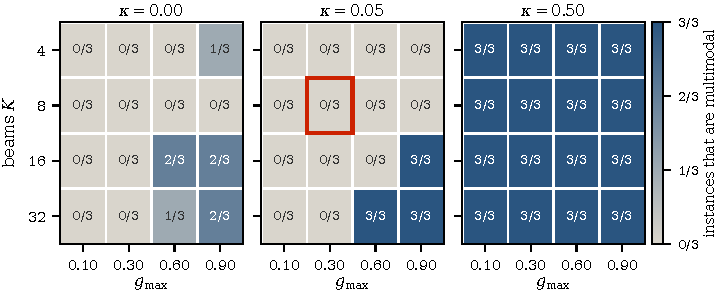
\includegraphics[width=\textwidth]{../figures/out/fig1-instance-space.pdf}
\caption{Instance space of the allocation problem. Each tile reports how many of the \numInst{}
instances at that configuration are multimodal. The outlined tile is the single configuration at
which an earlier screening run was performed.}
\label{fig:map}
\end{figure}

\subsection{Multimodality comes from amplifier distortion, not from interference}

Table~\ref{tab:knobs} breaks the map down by knob, and the structure is not what one would guess.
Beam count and interference strength both matter, but weakly: the multimodal fraction rises from
\numKnobKLo\% to \numKnobKHi\% across the range of $K$, and from \numKnobGmaxLo\% to
\numKnobGmaxHi\% across $g_{\max}$. The distortion term is different in kind. It moves the
fraction from \numKnobKappaLo\% to \numKnobKappaHi\%, and the movement is a step rather than a
gradient: the two lower levels behave alike and the highest level is multimodal everywhere.

\begin{table}[t]
\centering
\caption{Fraction of units that are multimodal, by knob and level. Distortion is the dominant
driver, and the two lower distortion levels are nearly indistinguishable.}
\label{tab:knobs}
\begin{tabular}{llrr}
\toprule
knob & level & units & multimodal (\%) \\
\midrule
$K$ & 4 & 36 & 36 \\
 & 8 & 36 & 33 \\
 & 16 & 36 & 53 \\
 & 32 & 36 & 58 \\
\midrule
$g_{\max}$ & 0.1 & 36 & 33 \\
 & 0.3 & 36 & 33 \\
 & 0.6 & 36 & 50 \\
 & 0.9 & 36 & 64 \\
\midrule
$\kappa$ & 0 & 48 & 17 \\
 & 0.05 & 48 & 19 \\
 & 0.5 & 48 & 100 \\
\bottomrule
\end{tabular}
\end{table}

This has a practical consequence for experiment design in this area. Interference strength is the
knob most often swept, because it is the one with an obvious physical interpretation for a
multi-beam system. It is not the knob that decides whether the optimisation problem is hard. A
sweep over $g_{\max}$ at low distortion explores a region that is overwhelmingly unimodal, and a
global search method evaluated there has nothing to demonstrate.

\subsection{All four optimisers, before splitting by region}

Table~\ref{tab:methods} reports the four optimisers over the whole grid, before any split by
region. Restart local search is best or tied in every unit. The two population baselines sit
below the QI method on mean rank, which is the comparison a paper in this area would typically
report and would typically report as a win.

\begin{table}[t]
\centering
\caption{All four optimisers over all \numUnits{} units. Mean rank is averaged over units, lower
being better. The last column is the median standard deviation across the \numSeeds{} seeds.}
\label{tab:methods}
\begin{tabular}{lrrr}
\toprule
method & best or tied & mean rank & median seed s.d. \\
\midrule
QI particle swarm & 65/144 & 2.25 & 0.0000 \\
CMA-ES & 50/144 & 2.50 & 0.0059 \\
Differential evolution & 27/144 & 3.56 & 0.0007 \\
Restart L-BFGS-B & 144/144 & 1.69 & 0.0000 \\
\bottomrule
\end{tabular}
\end{table}

\subsection{Position in the map decides the verdict}

Table~\ref{tab:verdict} and the left panel of Fig.~\ref{fig:verdict} cross the two arms. Restart
local search is best or tied in \numRestartBest{} of \numUnits{} units, and the QI method wins
\numQpsoWinTotal{} of them. That alone would be a familiar negative result. The structure behind
it is the part worth reporting.

\begin{table}[t]
\centering
\caption{QI method against restart local search, split by region of the instance space. The last
column is the absolute mean difference divided by the seed-induced standard deviation.}
\label{tab:verdict}
\begin{tabular}{lrrrrr}
\toprule
region & units & QI wins & tie & loss & effect / seed spread \\
\midrule
unimodal & 79 & 0 & 64 & 15 & 0.27 \\
multimodal & 65 & 0 & 1 & 64 & 0.70 \\
\bottomrule
\end{tabular}
\end{table}

\begin{figure}[t]
\centering
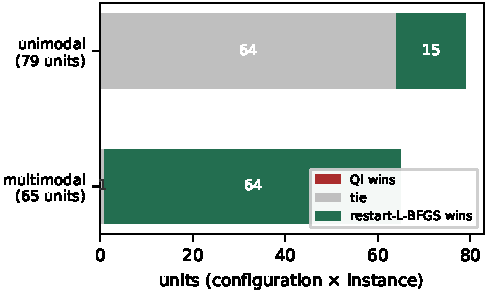
\includegraphics[width=0.49\textwidth]{../figures/out/fig2-verdict-by-region.pdf}
\hfill
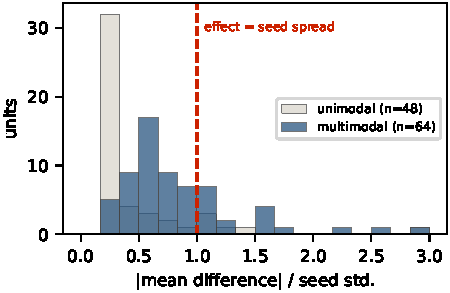
\includegraphics[width=0.49\textwidth]{../figures/out/fig3-effect-vs-seed-noise.pdf}
\caption{Left: outcome against restart local search, split by region of the map. Right:
distribution of the effect size in units of the seed-induced spread; the dashed line marks the
point at which a method difference equals the spread produced by changing the seed alone.}
\label{fig:verdict}
\end{figure}

On unimodal units the QI method \emph{ties} restart local search in \numUniTiePct\% of cases:
both find the same solution and the QI machinery buys nothing, because there is one basin and any
competent method reaches it. On multimodal units it \emph{loses} in \numMultiLossPct\% of cases.

This inverts the argument usually given for population-based search. Diversity is supposed to pay
on rugged landscapes. Here multimodality is not where diversity pays; it is where cheap restarts
pay. The reason is not mysterious. Sampling many basins independently is exactly what a restarted
local search does, and it does so at the cost of one convergence per basin, while a population
spends its budget maintaining a diversity it cannot convert into basin coverage at the same rate.

\subsection{Every effect is smaller than the seed spread, and no direction reverses}

The right panel of Fig.~\ref{fig:verdict} reports each method difference in units of the spread
caused by the seed alone. The median ratio is \numUniEffectRatio{} on unimodal units and
\numMultiEffectRatio{} on multimodal units. Both are below one: the difference between the two
methods is smaller than the difference one observes by changing the random seed and nothing else.

It would be wrong to read this as ``there is no effect''. The direction is perfectly consistent:
across all \numUnits{} units the QI method wins \numQpsoWinTotal{}. An ordering this stable but
this small is exactly the regime in which an underpowered study returns whichever answer its
seeds happened to give, and in which a single-seed study cannot be distinguished from a study
reporting noise. The next subsection quantifies that.

\subsection{What a study of the usual size would have concluded}

Figure~\ref{fig:under} reports \numStudies{} reconstructed studies of \numStudyCells{}
configurations and \numStudySeeds{} seeds each. Two findings follow, and the second is the one we
would ask readers to take away.

\begin{figure}[t]
\centering
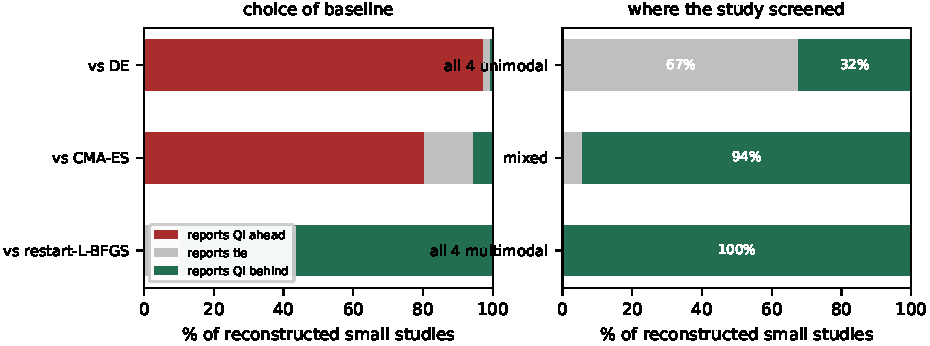
\includegraphics[width=\textwidth]{../figures/out/fig4-underpowered.pdf}
\caption{Verdicts of \numStudies{} reconstructed studies at the size usually reported. Left: the
verdict as a function of which baseline the study chose. Right: the verdict as a function of
where in the instance space the study happened to screen.}
\label{fig:under}
\end{figure}

\paragraph{The baseline decides the headline.}
Against differential evolution, \numSmallDeAhead\% of small studies report the QI method ahead.
Against CMA-ES, \numSmallCmaesAhead\% do. Against restart local search,
\numSmallRestartBehind\% report it behind. All three are faithful to the full data, which show
the QI method ahead of both population baselines and behind restart local search. No error is
involved and no bad faith is required: a paper that compares against a genetic algorithm and a
differential evolution baseline and reports a win is reporting something true. It is simply not
reporting the comparison that decides whether the method is worth deploying.

\paragraph{Where the study screened decides whether it sees anything at all.}
Among reconstructed studies whose \numStudyCells{} configurations all fell in the unimodal region
(\numAllUniN{} of \numStudies{}), \numAllUniTie\% report no difference between the QI method and
restart local search. Among those whose configurations all fell in the multimodal region
(\numAllMultiN{} of \numStudies{}), \numAllMultiBehind\% report the QI method behind. Same
problem, same methods, same budget, opposite headline, decided by a sampling choice that such
papers rarely state and never justify.

\paragraph{In fairness to the small design.}
Against restart local search the small design does mostly reach the correct direction, with only
\numSmallRestartAhead\% of studies reporting the QI method ahead. The failure mode here is not
that small studies invert the truth. It is that they resolve it into ``no difference''
\numSmallRestartTie\% of the time overall and \numAllUniTie\% of the time when they screen in the
easy region, and a reported non-difference is precisely what allows a method to remain in
circulation unexamined.

% =====================================================================
\section{Discussion}
\label{sec:discussion}

\subsection{Three things a paper in this area should report}

The results suggest three additions to reporting practice, all of them cheap.

\textbf{State where you screened, and screen more than one point.} The map in Fig.~\ref{fig:map}
took a few minutes of computation, far less than the optimiser comparison it contextualises. A
paper that reports the configurations it swept, and whether they are multimodal under a stated
criterion, gives a reader what is needed to judge whether the comparison had anything to detect.

\textbf{Include a restarted local search at matched budget.} It is the baseline a reviewer
reaches for first, it is trivial to implement, and in this problem it is the only baseline that
changes the conclusion. A comparison against population methods alone cannot distinguish ``this
QI method searches well'' from ``this problem does not need a population''.

\textbf{Report the effect against the seed spread.} A difference of a given size means something
different in a problem where seeds move the result by half that much than in one where they move
it by twice as much. The ratio costs nothing once repetitions exist, and it tells a reader
immediately whether the study had the resolution to see what it claims to have seen.

\subsection{What this does not say}

It does not say QI methods are useless for non-terrestrial resource allocation. It says that on
this problem, under this protocol, one QI method does not beat a restarted local search, and that
the published evidence pattern in this area would frequently not have detected that. A method
genuinely better would survive the same protocol, and the protocol would then be evidence in its
favour rather than an obstacle. That is the sense in which the contribution is intended as
constructive rather than negative.

Nor does it say small studies are unreliable in general. The reconstruction shows the opposite in
one respect: where an effect is consistent, a small design mostly recovers its direction. What
the small design loses is not the sign but the resolution, and with it the ability to tell a real
non-difference from an unexamined one.

\subsection{A note on generalisation}

The mechanism behind our central finding is not specific to this objective. Wherever multimodality
arises from a smooth nonlinearity on a boxed domain, basins are cheap to sample and a restarted
local search will be a strong baseline. We would expect the finding to weaken where basins are
expensive to reach, for example under integrality constraints or where evaluating the objective
requires a simulation rather than a closed form. That expectation is testable, and mapping the
instance space of such a problem is the way to test it.

% =====================================================================
\section{Threats to validity}
\label{sec:threats}

\textbf{One problem family, one generator.} The map is of one allocation problem under one
instance generator. Nothing here establishes how QI methods behave on scheduling, routing or
placement problems in the same networks, and the instance space of those problems would have to
be mapped separately. What transfers is the protocol; the verdict does not.

\textbf{The multimodality criterion is a choice.} Optima separated by less than \numMinSpread\%
of the best sum rate are treated as one basin. A stricter threshold would report more
multimodality and a looser one less. The threshold is stated rather than implied, and the
excluded non-finite and non-converged runs are counted rather than dropped silently, so a reader
can see the size of each exclusion.

\textbf{Restart local search is a baseline, not a recommendation.} That it wins here follows from
the geometry of this objective, which is smooth and box-constrained. It is the baseline a
reviewer reaches for first, which is why it is the one we ran. It is not a claim about what
should be deployed on a payload, where memory and code size constraints may exclude it.

\textbf{Budget is counted in evaluations, not wall-clock time.} Evaluation counting is the harder
constraint to satisfy and the easier one to verify, but it treats generously a method whose
per-call overhead is large. We report the evaluation budget rather than a timing comparison for
that reason, and a wall-clock study would be a useful complement.

\textbf{The reconstruction is resampling, not replication.} Section~\ref{sec:results} reports what
a small design would conclude \emph{given} that the full data describe the truth. It cannot speak
to a small study run on a different generator, and it creates no information the full data do not
already contain. It is a statement about the resolving power of a design.

\textbf{One QI variant.} We ran one quantum-inspired particle swarm method. Other QI families, in
particular quantum-inspired evolutionary algorithms with rotation-gate updates, may behave
differently, and this paper makes no claim about them.

% =====================================================================
\section{Conclusion}

Applying three established evaluation conventions together to one non-terrestrial allocation
problem changes what the evidence supports. A screening run at a single configuration can land in
the unimodal fraction of the instance space and conclude the opposite of what the map shows;
multimodality in this problem is created by amplifier distortion rather than by the interference
term that is usually swept; a budget-matched restart baseline is best or tied in
\numRestartBest{} of \numUnits{} units; and every effect we measure is smaller than the spread
the random seed alone produces, while its direction never once reverses.

Reconstructing \numStudies{} studies at the size usually reported shows why this matters in
practice. The headline such a study produces is governed by the baseline it chose and the region
it happened to sample, both decisions of the experimenter, neither customarily reported. The map
and the harness are released so the screening step can be run before a claim is made rather than
after it is disputed.

\subsubsection*{Reproducibility.} The instance space map, the raw per-seed results for all
\numUnits{} units, the reconstruction, and the harness that produced them are released with the
paper. Every number in this paper is generated from the released result files by a single
command; no result value is typed into the manuscript source.

\begin{thebibliography}{99}

\bibitem{restartfair}
Time-fair benchmarking for metaheuristics: a restart-fair protocol. arXiv:2509.08986 (2025)

\bibitem{greedyrestart}
Greedy restart schedules: a baseline for dynamic algorithm selection. arXiv:2504.11440 (2025)

\bibitem{benchbest}
Bartz-Beielstein, T., et al.: Benchmarking in optimization: best practice and open issues.
arXiv:2007.03488 (2020)

\bibitem{isa}
Smith-Miles, K., Baatar, D., Wreford, B., Lewis, R.: Towards objective measures of algorithm
performance across instance space. Comput. Oper. Res. \textbf{45}, 12--24 (2014)

\bibitem{isatools}
Smith-Miles, K., Mu\~noz, M.A.: Instance space analysis for algorithm testing: methodology and
software tools. ACM Comput. Surv. (2023)

\bibitem{isaqaoa}
On the instance dependence of optimal parameters for the quantum approximate optimisation
algorithm: insights via instance space analysis. arXiv:2401.08142 (2024)

\bibitem{seedrl}
Henderson, P., Islam, R., Bachman, P., Pineau, J., Precup, D., Meger, D.: Deep reinforcement
learning that matters. In: AAAI (2018)

\bibitem{seedllm}
Assessing the macro and micro effects of random seeds on fine-tuning large language models.
arXiv:2503.07329 (2025)

\bibitem{twovariances}
A tale of two variances: when single-seed benchmarks fail in Bayesian deep learning.
arXiv:2604.23114 (2026)

\bibitem{qideflation}
A released benchmark harness for the analysis of quantum-inspired search operators on synthetic
test functions. (Reference withheld for double-blind review; to be cited in the camera-ready.)

\end{thebibliography}

\end{document}
